\chapter{Implementation of A Resource Allocation Algorithm\label{cha:algorithm}}

This section describes the design and implementation of the \textit{QoS Scheduler Algorithm} which is used in section \ref{cha:orchestrator}. UML diagrams can be found in appendix \ref{cha:algorithm-UML-diagrams}.

\section{Algorithm architecture}

The algorithm takes an \texttt{Infrastructure} and an \texttt{Application} as inputs, and outputs an optimal deployment strategy (\texttt{AppDeployment}). Which strategy is optimal depends on the type of the scheduler. For example, the goal of a scheduler can be to minimize the total \textit{energy consumption}, the total \textit{network utilization} or the \textit{computing power} used. Since the focus here is on \textit{QoS}, the deployment that minimizes \textit{total latency} should be the optimal deployment. Figure \ref{fig:algorithm-architecture} illustrates the architecture of the algorithm.

\begin{figure}[h]
    \centering
    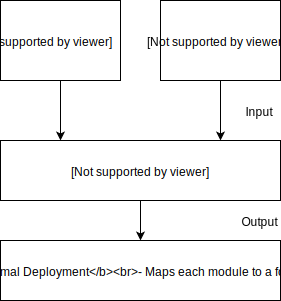
\includegraphics[width=7cm]{algorithm-architecture}
    \caption{QoS Scheduling algorithm architecture}
    \label{fig:algorithm-architecture}
\end{figure}


\subsection{Infrastructure\label{sec:algorithm-infrastructure}}

The infrastructure consists of \textit{fog nodes} and \textit{network connections} between those nodes. Network connections are modelled as uplinks only, because we are sending data forward in the application loop from one module to another, while every module is deployed on one fog node.
Between two nodes (node A and node B), the downlink of node B from node A's point of view is the same as the uplink of node A from node B's point of view. Therefore each fog node has a set of uplinks to all other reachable Fog nodes.
A node also has an uplink to itself, since the next module in the loop could be executed on the same node. This uplink is modeled with \textit{infinite speed} and \textit{zero latency}.
Thus, there are \(n^2\) uplinks in the infrastructure in total ($n \estimates number\ of\ Fog\ nodes$).
Figure \ref{fig:algorithm-infrastructure} shows a Fog infrastructure with three nodes and the corresponding nine uplinks.

\begin{figure}[htb]
    \centering
    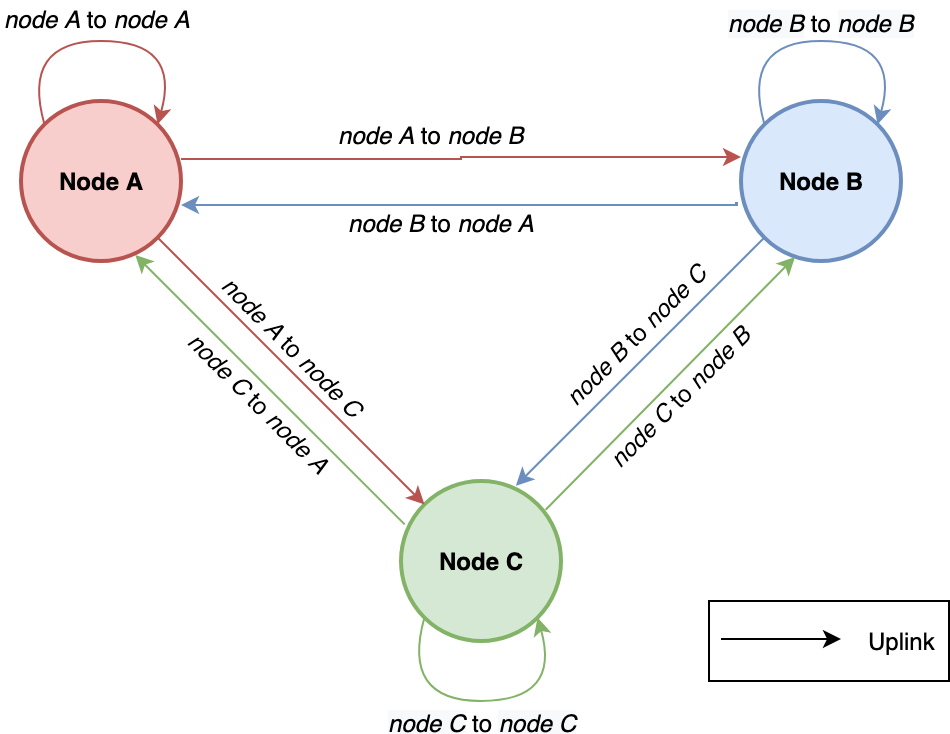
\includegraphics[width=0.75\textwidth]{algorithm-infrastructure}
    \caption{Infrastructure with three nodes and nine uplinks}
    \label{fig:algorithm-infrastructure}
\end{figure}

Next, the relevant classes for the infrastructure are described. The corresponding class diagram is depicted in figure \ref{fig:classdiagram-infrastructure}.

\begin{itemize}
    \item \underline{\texttt{Infrastructure}}: Contains a \texttt{List} of \texttt{FogNode} instances.
    
    \item \underline{\texttt{NetworkUplink}}: Every \texttt{NetworkUplink} instance has the following \textit{fields}:
    \begin{itemize}
        \item \underline{\texttt{source}}: The source \texttt{FogNode} of the link.
        \item \underline{\texttt{destination}}: The destination \texttt{FogNode} of the link.
        \item \underline{\texttt{latency}}: The RTT of the link.
        \item \underline{\texttt{bitPerSecond}}: The link speed (bandwidth) in bit per second.
    \end{itemize}

    \item \underline{\texttt{FogNode}}: Every \texttt{FogNode} instance has the following \textit{fields}:
    \begin{itemize}
        \item \underline{\texttt{id}}: The identifier of the device, e.g. hostname.
        \item \underline{\texttt{ramTotal}}: The total available ram.
        \item \underline{\texttt{storageTotal}}: The total available disk space.
        \item \underline{\texttt{cpuCores}}: The amount of available CPU cores.
        \item \underline{\texttt{cpuMips}}: The power of a CPU measured in MIPS (Million instructions per second).
        \item \underline{\texttt{connectedHardware}}: Hardware connected to the node (e.g. camera, temperature sensor)
        \item \underline{\texttt{uplinks}}: Uplinks to other fog nodes (instances of \texttt{NetworkUplink})
    \end{itemize}
    
    Every \texttt{FogNode} instance has the following \textit{methods}:
    \begin{itemize}
        \item \underline{\texttt{deployModule(AppSoftwareModule module): boolean}}\\ [0.5ex] 
        Tries to deploy an \texttt{AppSoftwareModule} (see section \ref{sec:algorithm-application}) on this node. Checks whether this node can fulfil the modules requirements (RAM, storage, hardware modules). Modules are \textit{not} automatically undeployed. The method can be called multiple times and thus more than one module can be deployed. In this case, sufficient resources must be available to execute \textit{all} modules. The method returns \texttt{false} for the first module that cannot be deployed, otherwise \texttt{true}.
        
        \item \underline{\texttt{getUplinkTo(FogNode destination): NetworkUplink}}\\ [0.5ex] 
        Returns the \texttt{NetworkUplink} from this node to the \texttt{destination} node.
        
        \item \underline{\texttt{calculateProcessingTime(AppSoftwareModule module): double}}\\ [0.5ex] 
        Calculates the execution time of an \texttt{AppSoftwareModule} (see section \ref{sec:algorithm-application}) on this node. Returns the value in milliseconds. The result is calculated using the following formula:
        \[\textrm{execution time [ms]} = \frac{\textrm{\texttt{requiredMi}}}{\textrm{\texttt{cpuMips}}}\ \boldsymbol{\cdot} 1000\]
    \end{itemize}

\end{itemize}


\subsection{Application\label{sec:algorithm-application}}

An application consists of \textit{modules}, \textit{messages} and \textit{loops}. A module can either be a \textit{hardware module} (e.g. a camera or a temperature sensor) or a \textit{software module} (e.g. data processor, object detection engine).

Next, the relevant classes for an application are described. The corresponsing class diagram is shown in figure \ref{fig:classdiagram-application}.

\begin{itemize}
    \item \underline{\texttt{AppModule}}: This abstract class is extended by the classes \texttt{AppHardwareModule} and \texttt{AppSoftwareModule}. It contains the the following \textit{fields}:
    \begin{itemize}
        \item \underline{\texttt{id}}: The type of this module, e.g. \texttt{CAMERA} (hardware) or \texttt{OBJECT\_DETECTOR} (software).
        \item \underline{\texttt{inputType}}: The modules input type, e.g. \texttt{IMAGE\_RAW} from a camera (can be \texttt{null} for the starting module of a loop).
        \item \underline{\texttt{outputType}}: The modules output type, e.g. \texttt{IMAGE\_PROCESSED} (can be \texttt{null} for the terminating module of a loop).
    \end{itemize}

    \item \underline{\texttt{AppHardwareModule}}: A hardware module extends \texttt{AppModule} and solely consists of the three fields of \texttt{AppModule}. If it has an \texttt{outputType} but no \texttt{inputType}, it is a \textit{sensor} (e.g. temperature sensor, outputs the current temperature). If it has an \texttt{inputType} but no \texttt{outputType}, it is an \textit{actuator} (e.g. air conditioner, takes a target value as input, outputs nothing).
    
    \item \underline{\texttt{AppSoftwareModule}}: A software module extends \texttt{AppModule} and additionally has the following \textit{fields}:
    \begin{itemize}
        \item \underline{\texttt{requiredRam}}: RAM required by the module.
        \item \underline{\texttt{requiredStorage}}: Disk storage required by the module.
        \item \underline{\texttt{requiredHardwareModules}}: Hardware modules that must be connected to the node that executes the software module. For instance, the hardware module \texttt{CAMERA} must be connected to a node which executes the software module \texttt{CAMERA\_CONTROLLER} in order to instruct the camera to take a picture first and output that picture to another module for further processing in the next step.
        \item \underline{\texttt{requiredMi}}: This attribute determines how many CPU instructions are needed approximately for processing a single message. This allows the execution time to be estimated.
    \end{itemize}
    
    \item \underline{\texttt{AppMessage}}: A message has the following \textit{fields}:
    \begin{itemize}
        \item \underline{\texttt{contentType}}: The content of a message, e.g. \texttt{IMAGE\_RAW}, \texttt{IMAGE\_PROCESSED}.
        \item \underline{\texttt{dataPerMessage}}: The data size per message in KByte, e.g. 500KB for an image.
    \end{itemize}
    A message has the following \textit{methods}:
    \begin{itemize}
        \item \underline{\texttt{transferTime(source: FogNode, destination: FogNode): double}}\\
        Calculates the transfer time of the message based on the \texttt{NetworkUplink} from \texttt{source} node to \texttt{destination} node. Returns the value in milliseconds. The result is calculated using the following formula:
        \[\textrm{transfer time [ms]} = \textrm{latency [ms]} + \frac{\textrm{message size [bit]}}{\textrm{link speed} [\frac{\textrm{bit}}{\textrm{ms}}]}\]
    \end{itemize}
   
   \item \underline{\texttt{AppLoop}}: A loop defines the connection between the different app modules. An application can consist of one or more loops, while each loop has a unique \textit{start}, \textit{end}, and \textit{maximum latency}. The loop determines how or in which \textit{order} the modules are \textit{connected} to each other. The maximum latency attribute defines the maximum allowed duration for one cycle. For instance, the loops last module \texttt{IMAGE\_VIEWER} should view an image not later than \textit{1 second} after the loops first module \texttt{CAMERA} took the image.
   
   In figure \ref{fig:object-detection-appmodules}, the order is as follows:\\
    \texttt{CAMERA} $\rightarrow$ \texttt{camera-controller} $\rightarrow$ \texttt{object-detector} $\rightarrow$ \texttt{image-viewer}\\[0.5ex]
   A loop has the following \textit{fields}:
   \begin{itemize}
       \item \underline{\texttt{name}}: The name of the loop, e.g. \textit{object-detection}.
       \item \underline{\texttt{maxLatency}}: Time (milliseconds) in which the result must be available, i.e. the time required to process all modules from the first to the last.
       \item \underline{\texttt{modules}}: A \texttt{LinkedList} containing all modules (IDs only) belonging to this loop. The order of this list determines the execution order of the loop.
   \end{itemize}
   A loop has the following \textit{methods}:
   \begin{itemize}
       \item \underline{\texttt{totalLatency(AppDeployment d): double}}\\
       Calculates the total latency for the loop for a given \texttt{AppDeployment} (see section \ref{sec:algorithm-scheduler}). Returns the value in milliseconds. The total latency is the sum of the loops task executions and its message transfers between modules. How these two values are calculated is depicted in figures \ref{fig:algorithm-activitydiagram-latency-processing} and \ref{fig:algorithm-activitydiagram-latency-transfer}.
   \end{itemize}
\end{itemize}

\begin{figure}[htbp]
    \centering
    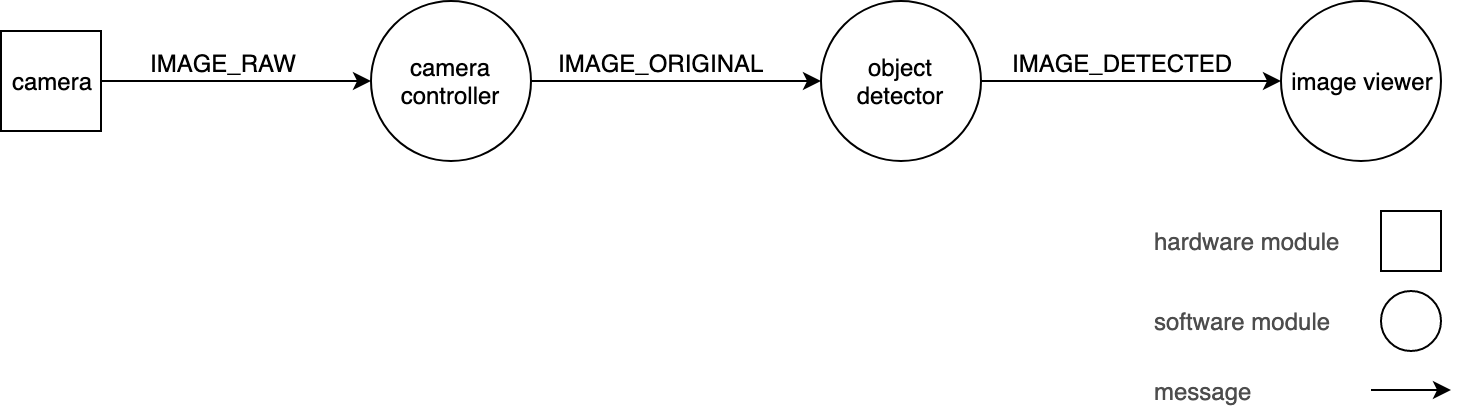
\includegraphics[width=1.0\textwidth]{object-detection-appmodules}
    \caption{Object detection application containing four modules}
    \label{fig:object-detection-appmodules}
\end{figure}

%%%%%%%%%%%%%%%%%%%%%%%%%%%%%%%%%%%%%%
%%%%% SUBSECTION INFRASTRUCTURE %%%%%%
%%%%%%%%%%%%%%%%%%%%%%%%%%%%%%%%%%%%%%


\subsection{Scheduler\label{sec:algorithm-scheduler}}

The architecture includes the interface \texttt{Scheduler}, which has the two methods \texttt{getOptimalDeployment()} and \texttt{getValidDeployments()}. The former method returns the one optimal deployment (\texttt{AppDeployment}), while the latter one returns a list of all possible deployments that meet the requirements. Class relationships are shown in figure \ref{fig:classdiagram-qosscheduler}.

The class \texttt{AppDeployment} is used to represent a deployment for a given \texttt{Application}. The field \texttt{moduleToNodeMap} is used to specify which module (\texttt{AppSoftwareModule}) should be executed on which node (\texttt{FogNode}).

In section \ref{sec:qos-scheduler} the concrete class \texttt{QosScheduler} is described, which implements the \texttt{Scheduler} interface.



\section{QoS Scheduler\label{sec:qos-scheduler}}
The job of the \textit{QoS scheduler} is to find all deployments which satisfy the latency requirements of all loops and output the one deployment with the lowest latency. How this task is solved is described in this section.\\

The \texttt{QosScheduler} takes an \texttt{Application} and an \texttt{Infrastructure} in the constructor. It tries to find all valid deployments as well as the optimal deployment for the \texttt{Application} over the \texttt{Infrastructure}. Figure \ref{fig:classdiagram-qosscheduler} shows the class diagram of the related classes.

In the first step the scheduler creates a combination of all possible deployment strategies without checking if the modules could be executed on the assigned nodes (hardware requirements) and if latency requirements are met (app loop requirements).
In a mathematical sense, a permutation with repetition is created in this step.

Table \ref{tab:deployment-combinations} shows all nine possible combinations of an application consisting of \textit{two modules} and an infrastructure consisting of \textit{three fog nodes}.

\begin{table}[htb]
    \centering
    \begin{tabular}{|c||c|c|}
    \hline
        \# & \textbf{module A} & \textbf{module B}\\
         \hline\hline
         1. & node 1 & node 1\\
         \hline
         2. & node 1 & node 2\\
         \hline
         3. & node 1 & node 3\\
         \hline
         4. & node 2 & node 1\\
         \hline
         5. & node 2 & node 2\\
         \hline
         6. & node 2 & node 3\\
         \hline
         7. & node 3 & node 1\\
         \hline
         8. & node 3 & node 2\\
         \hline
         9. & node 3 & node 3\\
         \hline
    \end{tabular}
    \caption{Combination of all possible deployments for an application with two modules and an infrastructure with three nodes}
    \label{tab:deployment-combinations}
\end{table}

Each line represents a \textit{deployment strategy candidate}, although it has not yet been checked whether the deployment strategy is valid because the requirements have not yet been checked. In order to do so, the \textit{QoS Scheduler} goes through several steps to check if a deployment strategy fulfills the application requirements. If the answer to any step is negative, this deployment strategy candidate is not valid and the next one will be checked. How the algorithm creates a set of valid deployments is depicted in \ref{fig:algorithm-activitydiagram-validdeployments}, which is also the implementation of the method \texttt{getValidDeplopyments()}.

\begin{figure}[htb]
    \centering
    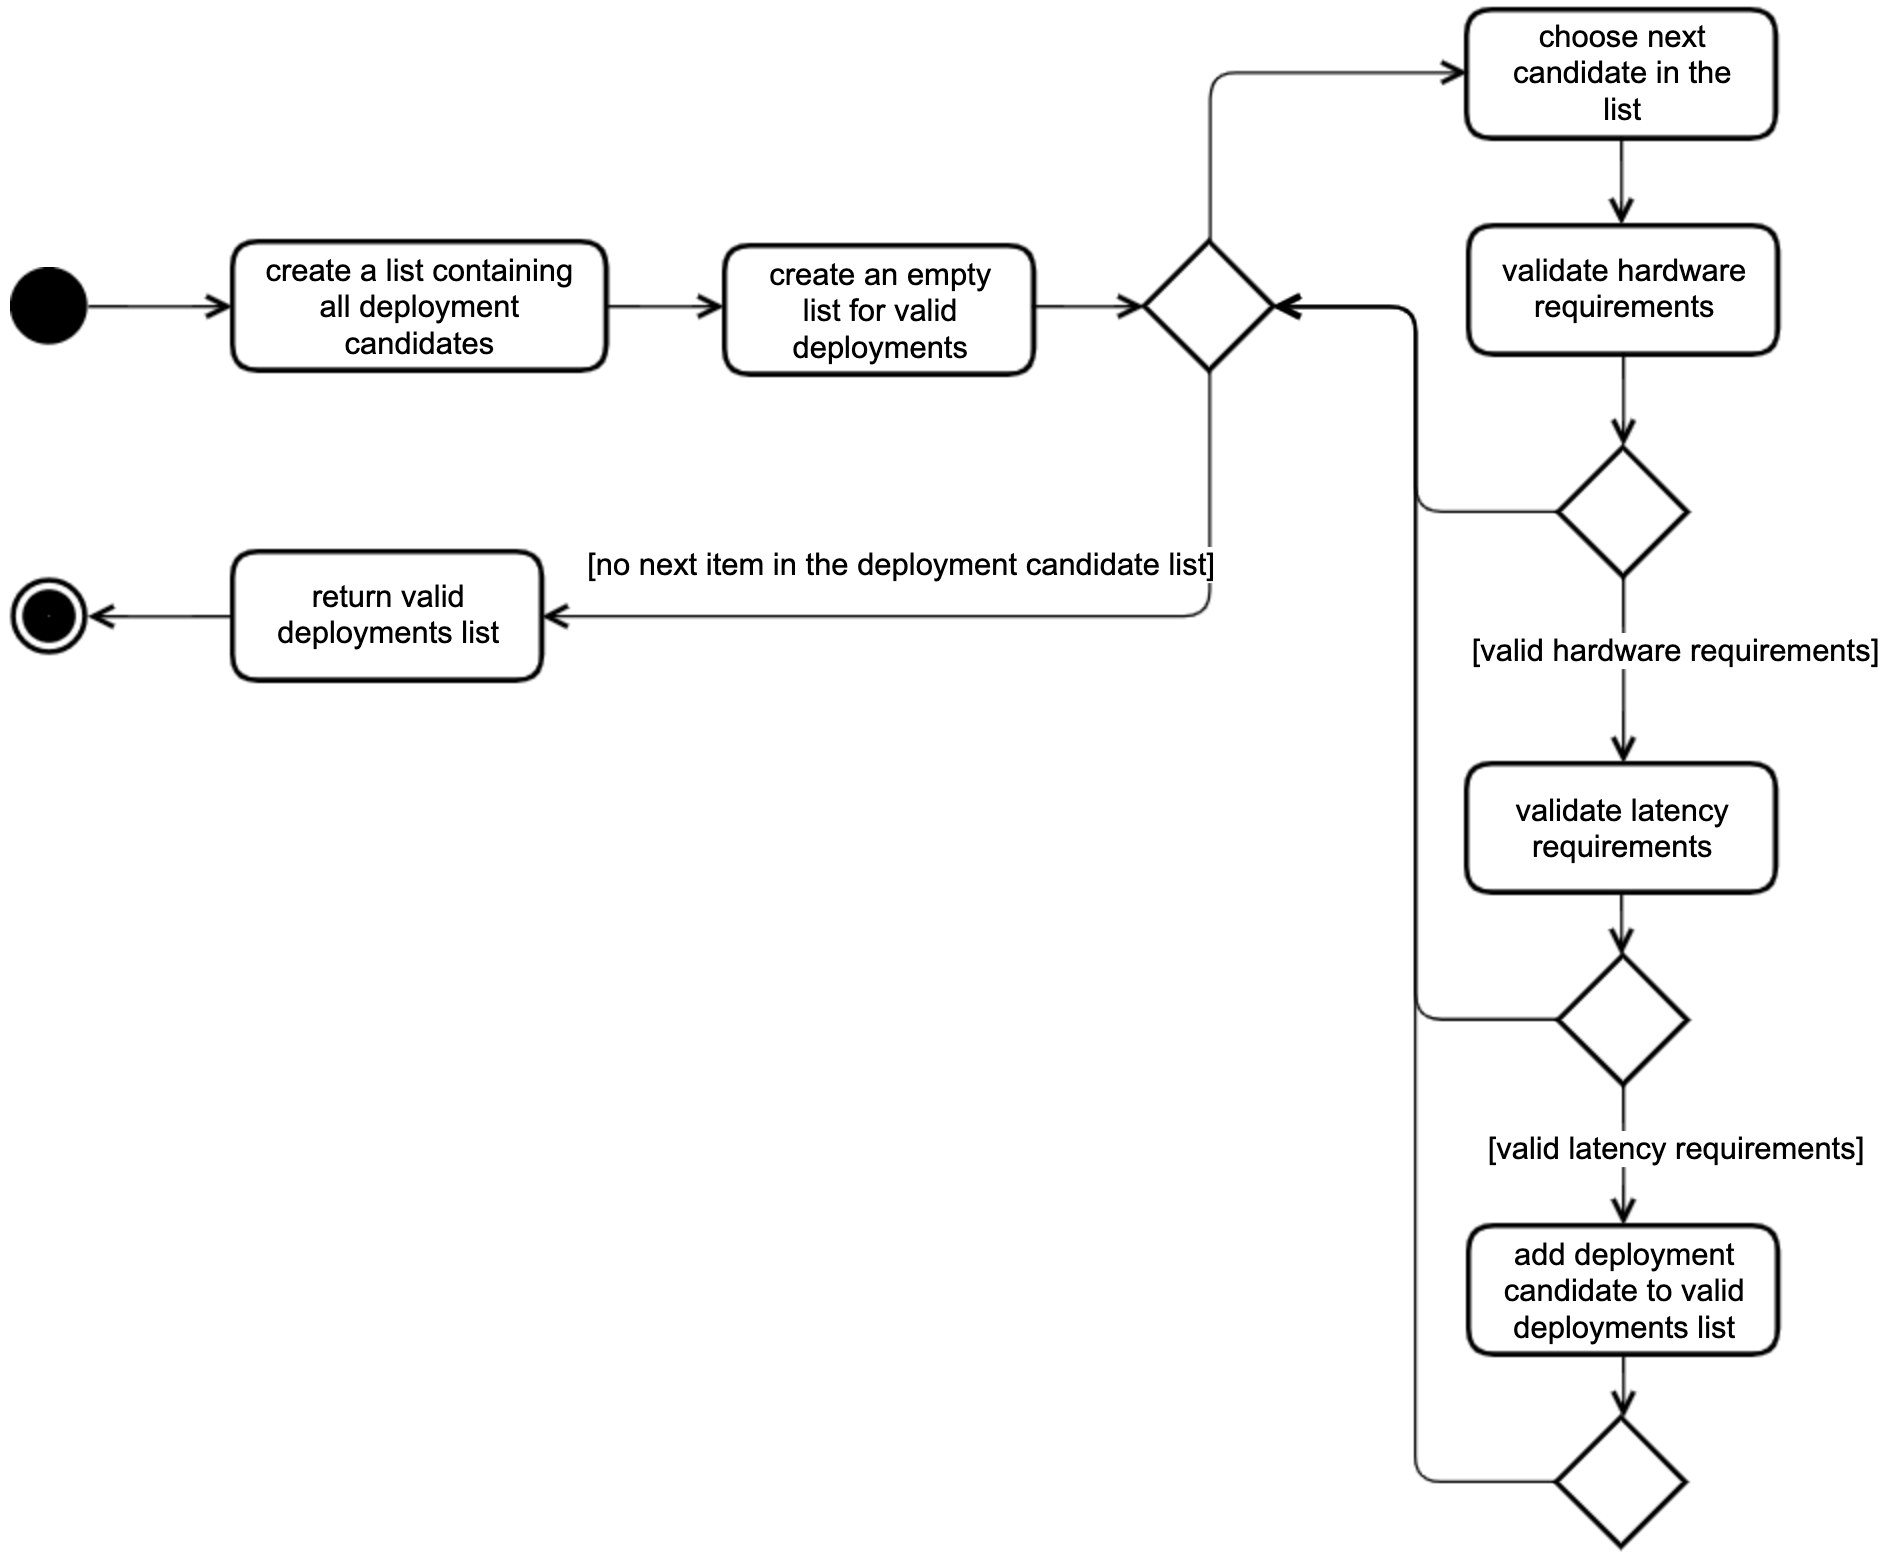
\includegraphics[width=1.0\textwidth]{algorithm-activitydiagram-validdeployments}
    \caption{Activity diagram for finding possible deployments}
    \label{fig:algorithm-activitydiagram-validdeployments}
\end{figure}

The result is a set of deployments which fulfill the application requirements. The \textit{optimal deployment} is the one with the \textit{lowest total latency} and will be returned by calling the method \texttt{getOptimalDeployment()}. The corresponding activity diagram is shown in figure \ref{fig:algorithm-activitydiagram-optimaldeployment}.

\begin{figure}[htb]
    \centering
    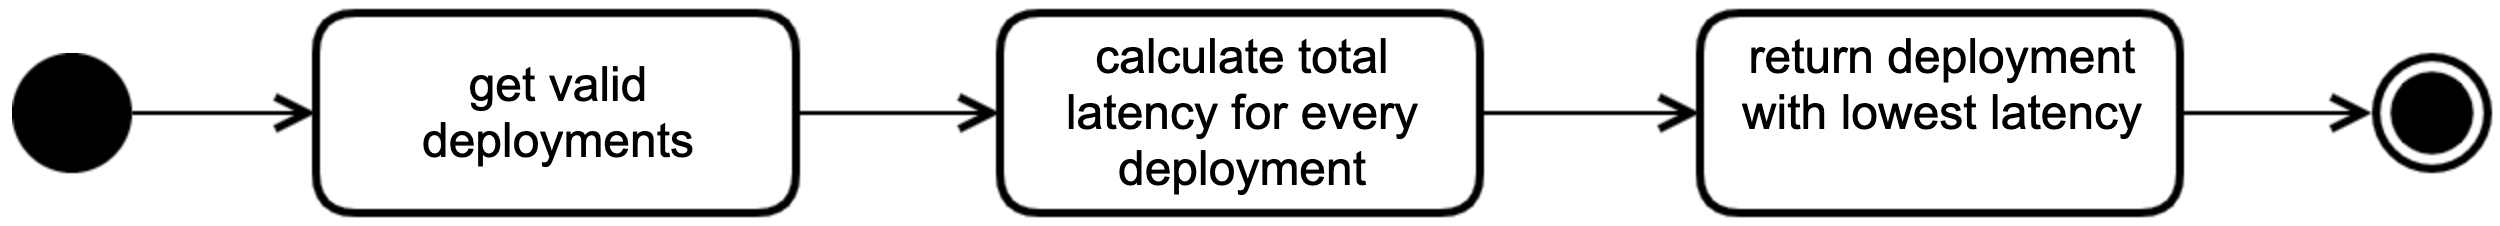
\includegraphics[width=1.0\textwidth]{algorithm-activitydiagram-optimaldeployment}
    \caption{Activity diagram for finding the optimal deployment}
    \label{fig:algorithm-activitydiagram-optimaldeployment}
\end{figure}

How the hardware and latency requirements are validated is shown in figures \ref{fig:algorithm-activitydiagram-hardware} and \ref{fig:algorithm-activitydiagram-latency}. To validate latency requirements it is necessary to calculate the \textit{total latency} of a loop, which is the sum of the processing times of all modules and all message transfers between the modules of the loop. The following formula shows the calculation of the total latency with $t_n$ = execution time of module \textit{n} and $t_m$ = transfer time of message \textit{m}:

\[ \textrm{total latency} = \sum_{n=0}^N t_n + \sum_{m=0}^M t_m\]

The calculations of \textit{total processing time} and \textit{total transfer time} are depicted in activity diagrams in figures \ref{fig:algorithm-activitydiagram-latency-processing} and \ref{fig:algorithm-activitydiagram-latency-transfer}.

